\section{Results}
Results!

\begin{figure}[t]
\centering
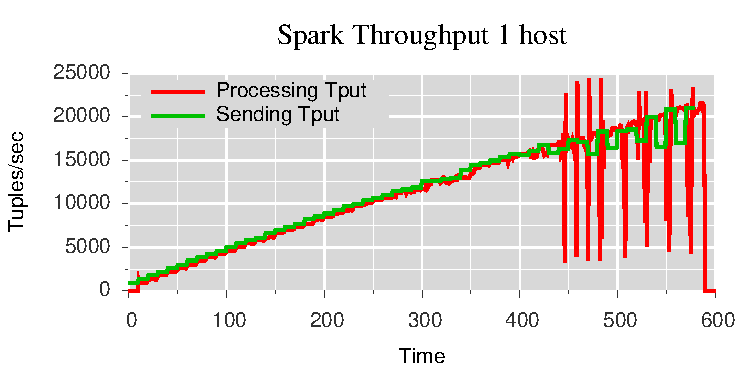
\includegraphics[width=1\linewidth]{figures/sp1_tput.pdf}
%\vspace{-0.3in}
\caption{Throughput/Time for a single Spark host running word count. We sent 100B tuples at a
slowly ramped up rate from 1K tuples/sec to 30k tuples/sec with a step size of
500 tuples/sec. The sending rate remained constant for 10 seconds before
transitioning to the next throughput.}
\label{fig:sb1-tput}
\end{figure}

\begin{figure}[t]
\centering
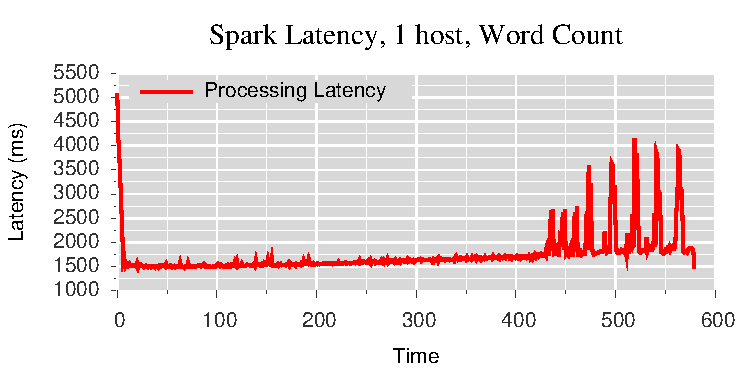
\includegraphics[width=1\linewidth]{figures/sp1_latency.pdf}
%\vspace{-0.3in}
\caption{Average latency to process tuples for a single Spark host. Similar to
Figure~\ref{fig:sb1-tput} we sent 100B tuples at a slowly ramped up rate from 1K
tuples/sec to 30k tuples/sec with a step size of 500 tuples/sec. The sending
rate remained constant for 10 seconds before transitioning to the next
throughput. The astute reader will notice that the latency spike in this graph
occurs at the same time as the loss in throughput consistency in
Figure~\ref{fig:sb1-tput}.}
\label{fig:label-me-if-you-want}
\end{figure}

\begin{figure}[t]
\centering
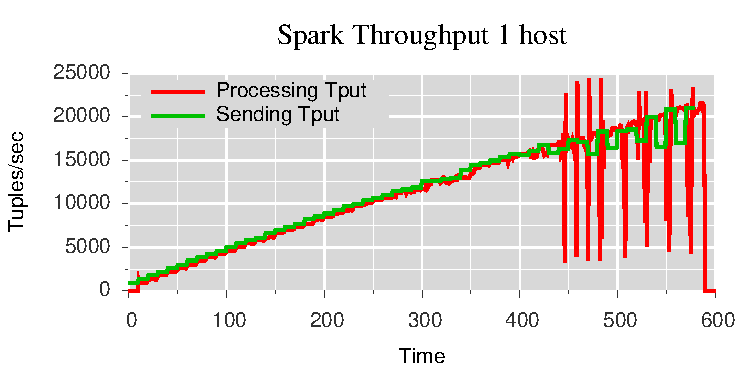
\includegraphics[width=1\linewidth]{figures/sp1_tput.pdf}
%\vspace{-0.3in}
\caption{Throughput/Time for a single Spark host, running grep. We sent 100B tuples at a
slowly ramped up rate from 1K tuples/sec to 30k tuples/sec with a step size of
500 tuples/sec. The sending rate remained constant for 10 seconds before
transitioning to the next throughput.}
\label{fig:sb1-tput}
\end{figure}

\begin{figure}[t]
\centering
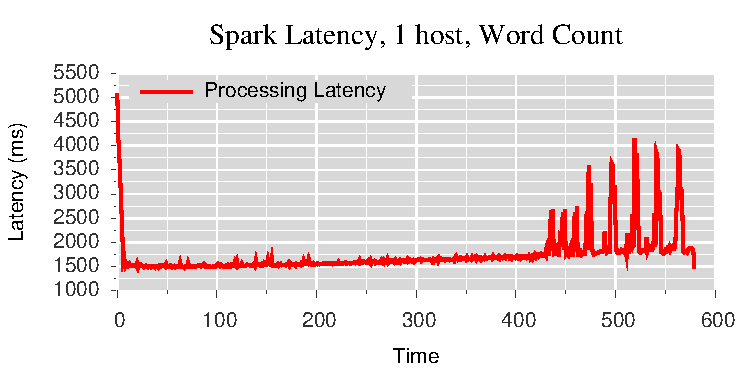
\includegraphics[width=1\linewidth]{figures/sp1_latency.pdf}
%\vspace{-0.3in}
\caption{Average latency to process tuples for a single Spark host. Similar to
Figure~\ref{fig:sb1-tput} we sent 100B tuples at a slowly ramped up rate from 1K
tuples/sec to 30k tuples/sec with a step size of 500 tuples/sec. The sending
rate remained constant for 10 seconds before transitioning to the next
throughput. The astute reader will notice that the latency spike in this graph
occurs at the same time as the loss in throughput consistency in
Figure~\ref{fig:sb1-tput}.}
\label{fig:label-me-if-you-want}
\end{figure}



\begin{figure}[t]
\centering
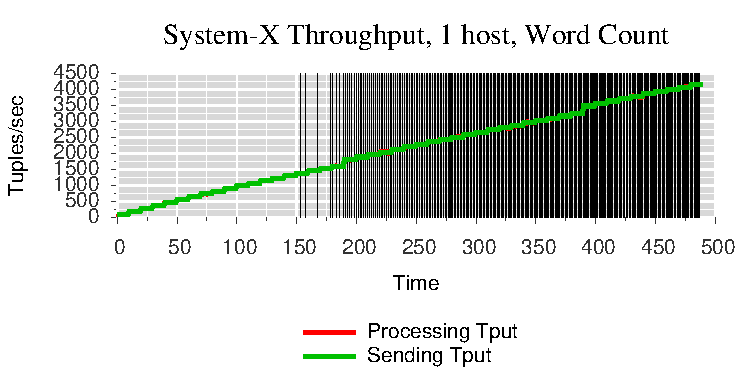
\includegraphics[width=1\linewidth]{figures/sb1_tput.pdf}
%\vspace{-0.3in}
\caption{System-X word count. The black vertical bars represent System-X producing errors relating to it unable to transform the bytes in its internal buffer to a tuple.}
\label{fig:label-me-if-you-want}
\end{figure}

\begin{figure}[t]
\centering
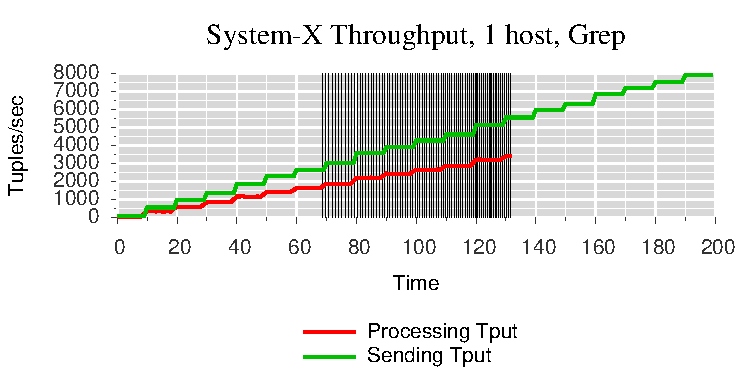
\includegraphics[width=1\linewidth]{figures/sb2_tput.pdf}
%\vspace{-0.3in}
\caption{System-X grep. Around time step 130 System-X froze and would not report anymore results but somehow kept the TCP connection with the tuple generator alive since it was happy to keep receiving tuples but dropping them on the floor.}
\label{fig:label-me-if-you-want}
\end{figure}


\begin{figure}[t]
\centering
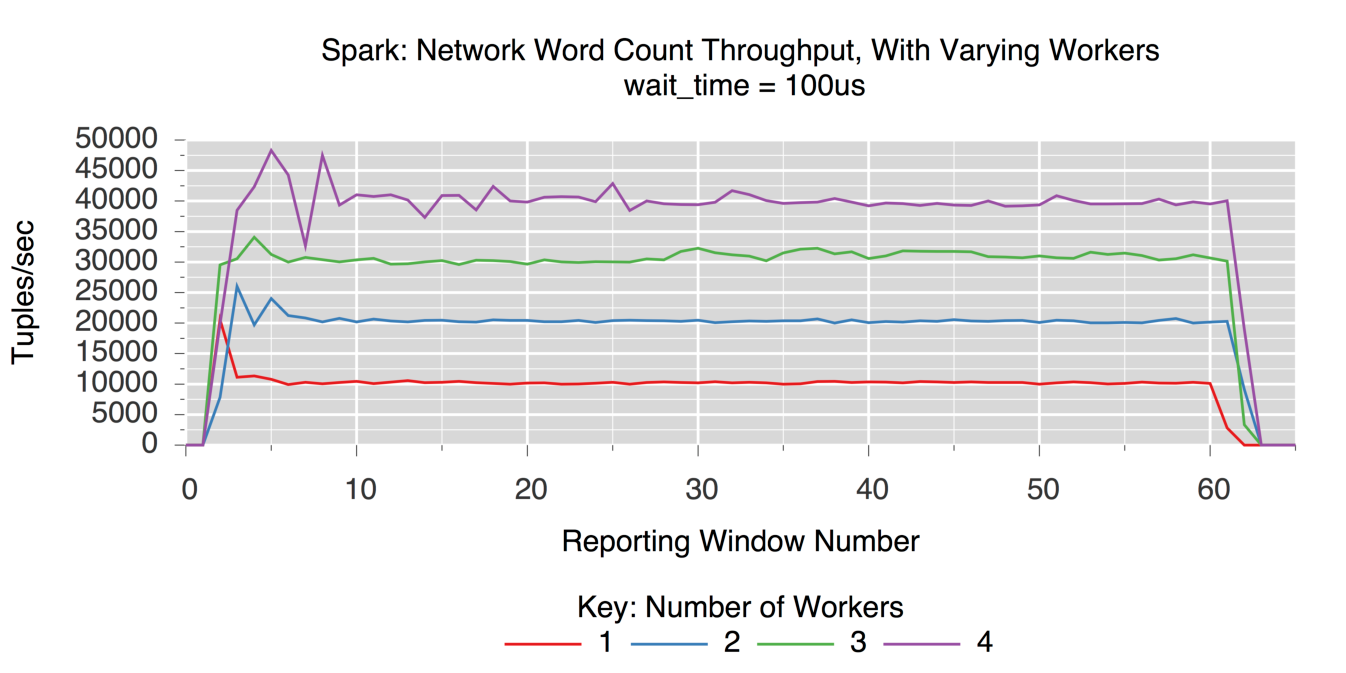
\includegraphics[width=1\linewidth]{figures/spark-wc-dist.pdf}
%\vspace{-0.3in}
\caption{Spark distributed, word count}
\label{fig:label-me-if-you-want}
\end{figure}


\begin{figure}[t]
\centering
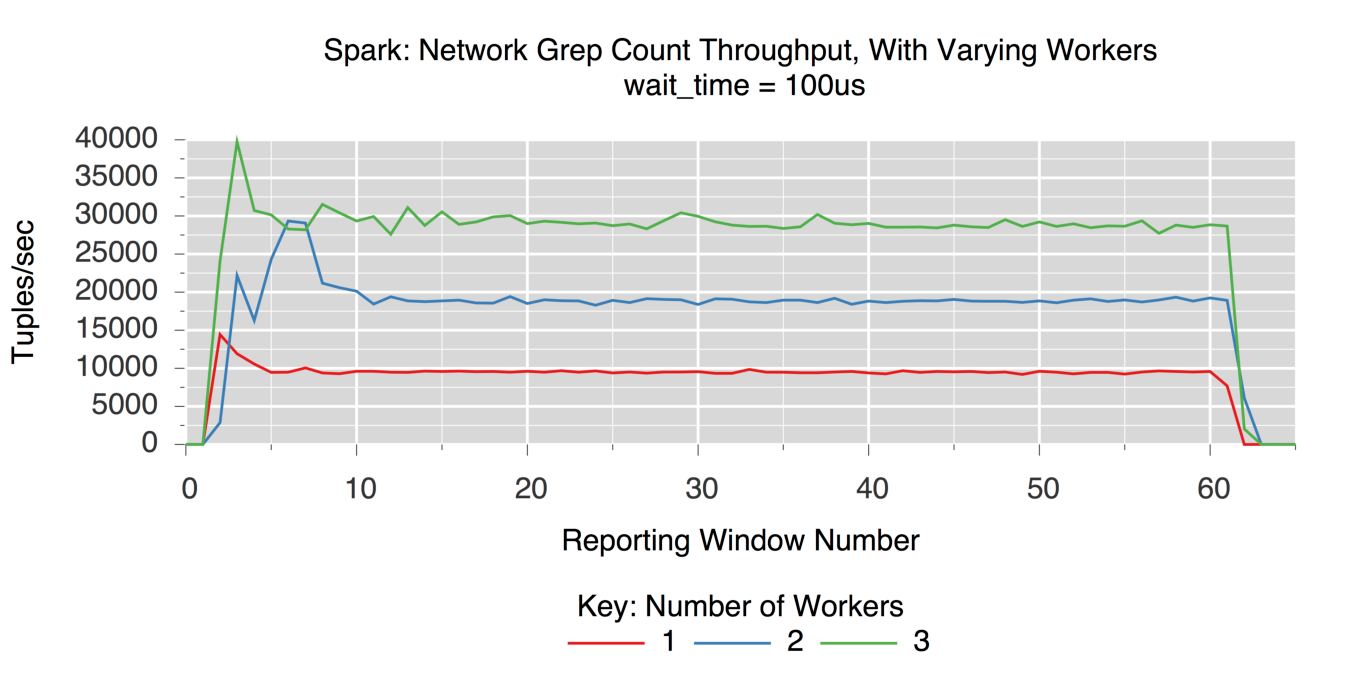
\includegraphics[width=1\linewidth]{figures/spark-grep-dist.pdf}
%\vspace{-0.3in}
\caption{Spark distributed, grep}
\label{fig:label-me-if-you-want}
\end{figure}




